\kommentar{Leitungen}

\begin{karte}{Was ist eine Leitung?}
	Für uns ist eine Leitung eine Wellenführung.\\
	\divTwo{
		\textbf{Ungeführte Welle:}
		%Autor: Simon Walker
%Version: 1.0
%Datum: 24.04.2020
%Lizenz: CC BY-NC-SA

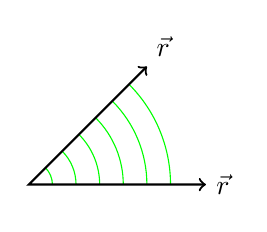
\begin{tikzpicture}[smooth, xscale=0.5, yscale=0.5]
	%\HelpCords{0}{0}{5}{4}
	
	\foreach \x in {0.6, 1.2, ...,4}{
		\draw[green] (\x, 0) arc (0:45:\x);	
	}
	
	\draw[<->, thick] (3, 3) -- (0, 0) -- (4.5, 0) node[right] {$\vec{r}$};
	\node[above right] at (3, 3) {$\vec{r}$};
\end{tikzpicture}
\\
		\scalebox{.7}{%Autor: Simon Walker
%Version: 1.0
%Datum: 24.04.2020
%Lizenz: CC BY-NC-SA

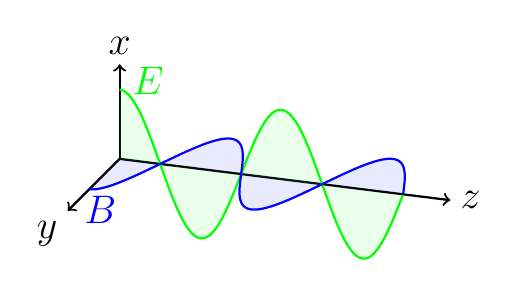
\begin{tikzpicture}[x={(0,0.8cm)}, y={(-0.55cm,-0.55cm)}, z={(1.2cm, -0.15cm)}]
		
	\def\cycles{1.75} %Anz Schwingungen
	\def\lenght{3}%länge in z richtung
	
	
	\draw [->, thick] (0,0,0)  -- (1.5,0,0) node[above] {\Large$x$};
	\draw [->, thick] (0,0,0) -- (0,1.2,0) node[below left] {\Large$y$};
	\draw [->, thick] (0,0,0) -- (0,0,\lenght+0.5) node[right] {\Large$z$};
	
	\draw[thick, green] %E-Feld Plot
	plot[domain=0:\lenght, samples=200] 
	({1.1*cos(deg(2*\cycles*pi*\x/\lenght))}, 0, \x);
	
	\draw[thick, blue] %M-Feld Plot
	plot[domain=0:\lenght, samples=200] 
	(0, {0.7*cos(deg(2*\cycles*pi*\x/\lenght))}, \x);
	
	\fill[opacity=.1,green!80] %E-Feld füllung
	(0,0,0) --
	plot[domain=0:\lenght, samples=200] 
	({1.1*cos(deg(2*\cycles*pi*\x/\lenght))}, 0, \x)  --
	(0,0,0);
	
	\fill[opacity=.1,blue!80] %M-Feld füllung
	(0,0,0) --
	plot[domain=0:\lenght, samples=200] 
	(0, {0.7*cos(deg(2*\cycles*pi*\x/\lenght))}, \x)  --
	(0,0,0);
	
	\node[green] at (1.3,0,0.3) {\Large$E$}; %Beschriftungen
	\node[blue] at (0,1.1,0.3) {\Large$B$};
	
\end{tikzpicture}
}
		\centering
		$\vec{k} \cdot \vec{r}$
		
	}{
		\textbf{Geführte Welle:}\\[5pt]
		%Autor: Simon Walker
%Version: 1.0
%Datum: 24.04.2020
%Lizenz: CC BY-NC-SA

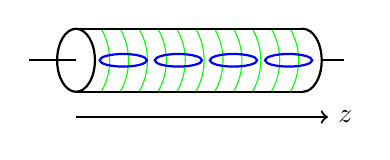
\begin{tikzpicture}[smooth, xscale=0.4, yscale=0.4]
%	\HelpCords{0}{-1}{9}{1}

	\draw[thick] (-0.5, 0) -- (1, 0);
	\draw[thick] (8, 0) -- (9.5, 0);
	
	\draw[thick] (1, 0) ellipse circle [x radius=0.6, y radius=1];
	
	\draw[thick, fill=white] (8.2, 0) ellipse circle [x radius=0.6, y radius=1];
	\fill[white] (7,-1) rectangle (8.2,1);
	
	\foreach \x in {1.8, 2.4, ...,8}{
		\draw[green] (\x, -1) arc (-30:30:2);	
	}
	
	\draw[thick] (1, 1) -- (8.2, 1);
	\draw[thick] (1, -1) -- (8.2, -1);
	
	\foreach \x in {2.5, 4.25, ..., 8}{
		\draw[thick, blue] (\x, 0) ellipse circle [x radius=0.75, y radius=0.2];
	}

	\draw[thick, ->] (1, -1.8) -- (9, -1.8) node[right] {$z$};
\end{tikzpicture}

		\begin{center}
			$k\cdot z = \beta z \quad \Rightarrow \quad k=\beta$
		\end{center}
		Im Beispiel ist ein Koaxialleiter zu sehen. Das $B$-Feld ist Ortogonal zum $E$-Feld. Die gesamte Anordnung ist Symetrisch.
	}
\end{karte}

\begin{karte}{Was ist eine TEM-Welle?}
	TEM steht für transversalelektomagnetisch. Eine TEM-Welle hat nur Komponenten, welche senkrecht zur Ausbreitungsrichtung sind.\\[10pt]
	%Autor: Simon Walker
%Version: 1.0
%Datum: 28.04.2020
%Lizenz: CC BY-NC-SA

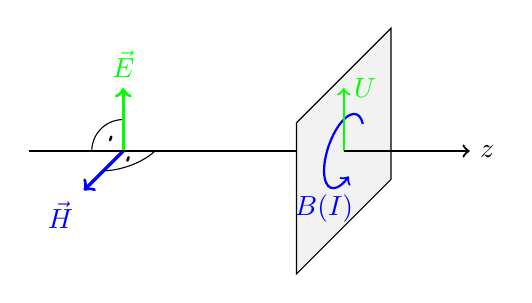
\begin{tikzpicture}[x={(0, 0.8cm)}, y={(-0.5cm,-0.5cm)}, z={(0.8cm, 0)}]

\def\l{7} %länge der z-Achse
\def\s{1.2} %Quadratgrösse (eine Seite ist s*2)
\def\p{5} %Positoon des Quadrates

\draw[domain=90:180,smooth,variable=\x] plot ({sin(\x)*0.5},{0}, {1.5+cos(\x)*0.5});
\draw[domain=0:90,smooth,variable=\x] plot ({0},{sin(\x)*0.5}, {1.5+cos(\x)*0.5});
\draw[fill=black] (0.2, 0, 1.3) circle[radius=0.03];
\draw[fill=black] (0, 0.2, 1.7) circle[radius=0.03];
\draw[very thick, green, ->] (0, 0, 1.5) -- (1, 0, 1.5) node[above, green] {$\vec{E}$};
\draw[very thick, blue, ->] (0, 0, 1.5) -- (0, 1, 1.5) node[below left, blue] {$\vec{H}$};

\draw[thick] (0, 0, 0) -- (0, 0, \p); %Beginn der Z-Achse

\draw[fill=gray!10] (-\s, -\s, \p) -- (-\s, \s, \p) -- (\s, \s, \p) -- (\s, -\s, \p) -- cycle;
\draw[->,domain=-75:195,smooth,variable=\x, blue, thick] plot ({cos(\x)*0.5},{sin(\x)*0.5}, {\p});
\node[blue] at (-0.6, 0.5, \p) {$B(I)$};
\draw[->, green, thick] (0, 0, \p) -- (1, 0, \p) node[right, green] {$U$};
\draw[thick, ->] (0, 0, \p) -- (0, 0, \l) node[right] {$z$}; %Ende der Z-Achse

\end{tikzpicture}

\end{karte}
